\begin{figure}[ht!]
    \centering
    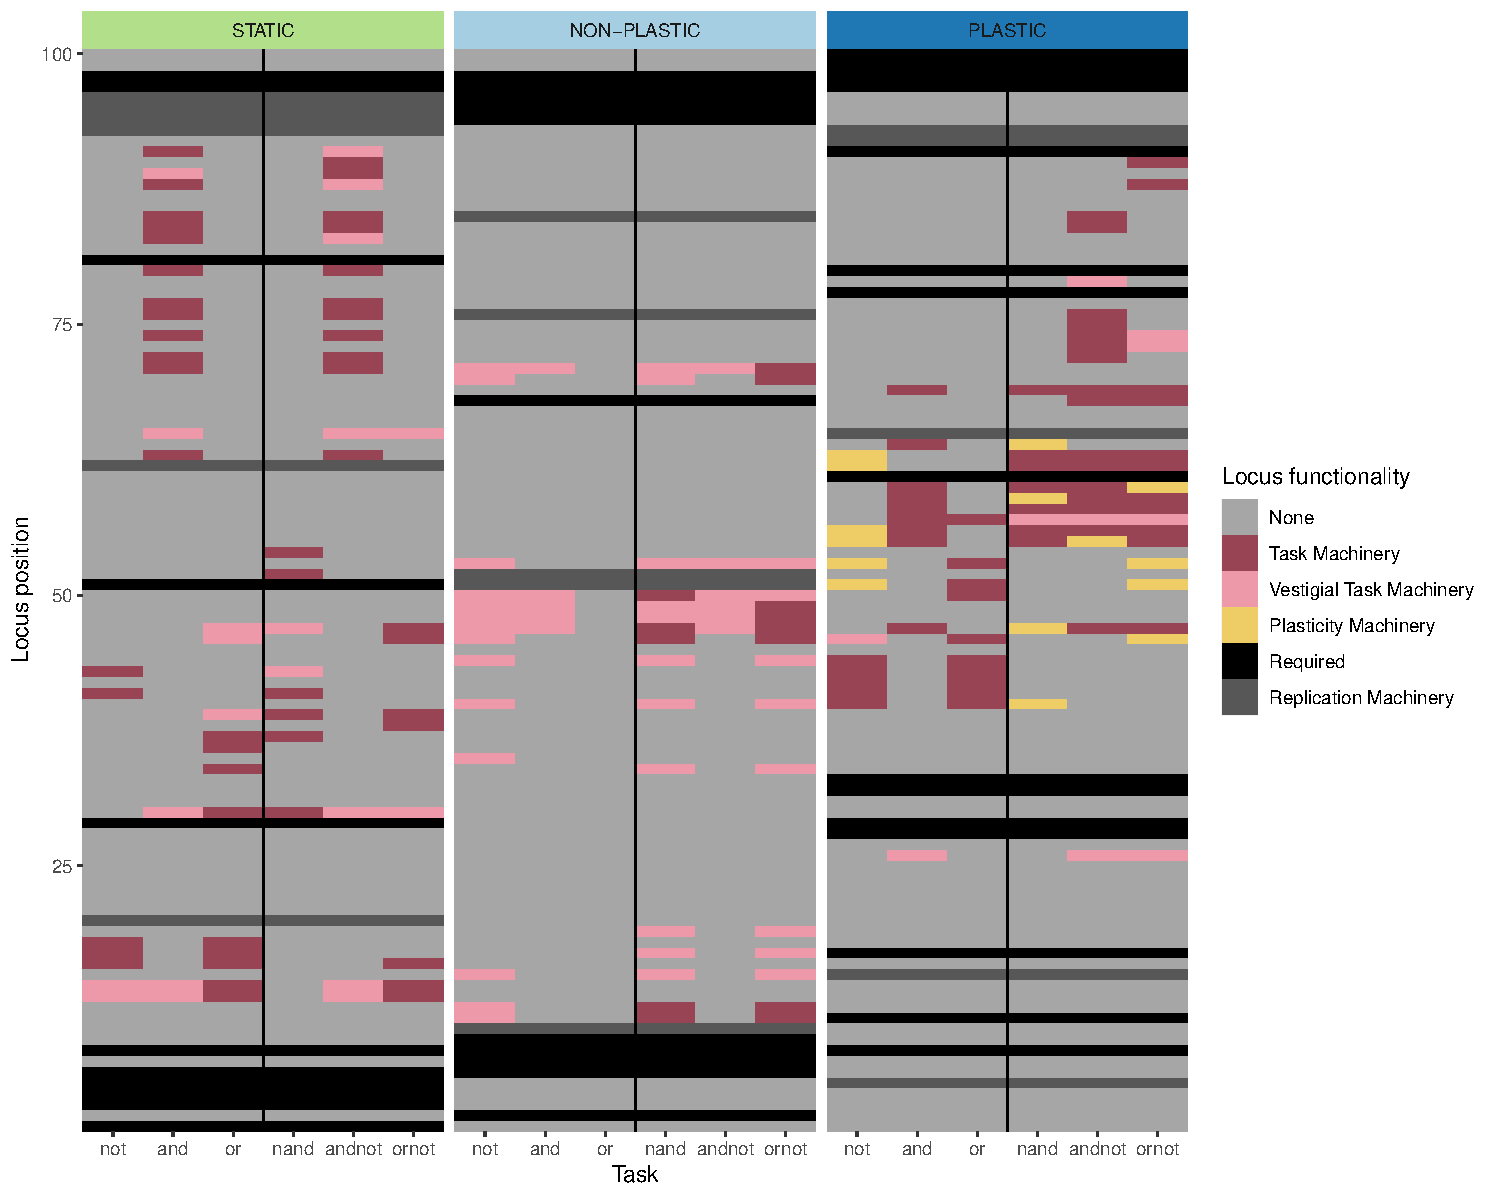
\includegraphics[width=1\textwidth]{chapters/03-evolutionary-consequences-of-plasticity/media/locus-slice-combined-color-facets.pdf}
    \caption{\small
    \textbf{Representative genetic architectures from each treatment.}
    Each box shows a representative genome from each condition at the end of Phase 2A. 
    The y-axis indicates each site in each genome, and colors indicate the function of each locus with respect to a particular task (given by the x-axis). 
    % Each of the six base tasks are shown on the x axis. 
    The vertical black line splits tasks rewarded in ENV-A (left of the line) from those rewarded in ENV-B.
    Loci colored as ``Task Machinery'' are actively involved in the performance of that task, while ``Vestigial Task Machinery'' represents loci that have not mutated, but no longer code for the task (\textit{i.e.}, a change elsewhere in the genome has disabled or modified the task). 
    ``Plasticity Machinery'' refers to loci that regulate the given task. 
    Knocking out a ``Replication Machinery'' locus negatively affects replication time, while knocking out a ``Required'' locus results in a non-viable organism. 
    }
    \label{chapter:consequences-of-plasticity:fig:architecture-locus-functionality}
\end{figure}